\documentclass[11pt]{l3deliverable}
\usepackage[table]{xcolor}
\usepackage{geometry}
\usepackage{fullpage}
\usepackage{graphicx}
\usepackage{tabularx}
\usepackage{hyperref}
\usepackage{xcolor}
\newcolumntype{T}{>{\centering\arraybackslash}m{0.20\textwidth}}
\newcolumntype{L}{>{\centering\arraybackslash}m{0.74\textwidth}}
\definecolor{medium-red}{rgb}{0.35,0,0}
\hypersetup{colorlinks, linkcolor={medium-red}, citecolor={medium-red},
urlcolor={medium-red}}
\geometry{a4paper}
\setlength\parindent{0pt}
\title{Change Report}
\deliverableID{D8.3}
\project{PSD3 Group Exercise 2}
\team{W}
\version{1.0}
\author{
    Gordon Reid: 1002536R\\
    Ryan Wells: 1002253W\\
    Kristopher Stewart: 1007175S\\
    David Selkirk: 1003646S\\
    James Gallagher: 0800899G\\
}
\date{\today}

\begin{document}

\maketitle

\newpage

\tableofcontents

\newpage

\section{Introduction}

\subsection{Identification}

This is the change report completed by Team W detailing changes to the 
internship management system. The internship management system is for 
Software Engineering (SE) and Electronic and Software Engineering (ESE) 
students, studying in the School of Computing Science.

\subsection{Related Documentation}

D8.4 Task Description:

\url{http://fims.moodle.gla.ac.uk/file.php/128/coursework/maintenance_d8.4.pdf}

PSD3 Group Exercise Description:

\url{http://fims.moodle.gla.ac.uk/file.php/128/coursework/psd3-ge-2.pdf}

PSD3 Requirements Specification:

\url{fims.moodle.gla.ac.uk/file.php/128/coursework/requirements-specification-ge2.pdf}

\subsection{Purpose and Description Of Document}

This document serves as the Change Report based on the updated requirements
detailed in the D8.4 handout. 

\newpage

\section{Major Changes}

\subsection{Student and StudentImpl}

The most fundamental change in the internship management system was altering the
number of internships a student could have. This required several key changes
in the Student interface and the StudentImpl class that implements this interface.
First and foremost, the single internship stored in a student object was replaced 
with a HashMap of internships. This was modelled after the way the adManager stores
adverts, complete with a counter that both counts the number of internships have been 
accepted and allows us to return the most recently accepted internship (vital for the 
InternMan method approveAcceptedOffer()). The Student now returns the HashMap of 
internships rather than the single one. Adding an internship now checks that the new
internship does not overlap any of the students existing ones, as per the change 
specifications. Similarly, a private method was created that calculates whether a
student has enough internships to fill 12 weeks and a getter created to return the 
results of this method. The abstraction here was to keep the public methods relatively
short and readable.

\subsection{AdminInterface and Admin}

The change in the way we get internships had various ripple effects throughout the 
system. The method approveOffer(String matriculation) was extended with an Integer
identifier parameter to allow the user to specify which internship to approve. The 
method assignAcademicVisitor() was also altered to set the visitor in every one of
the students internships, as the documentation states that for a student all 
internships will have the same visitor. RecordVisitorAssessment() was changed such
that it adds the information to the most recently accepted internship.

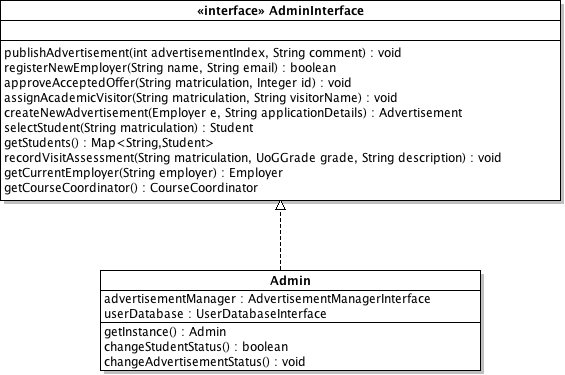
\includegraphics[width=\textwidth]{adminClassDiagram.png}

\subsection{InternManTeamW}

The changes to this class were minor. createNewSelfSourcedRole() submits the role to
the first internship in the students map and approveAcceptedOffer()'s javadoc was 
expanded. 

\subsection{Test Cases}

The ApproveAcceptedOffer, NotifyAcceptedOffer and ViewStudentDetail test cases all 
needed slight modifications to deal with the change to StudentImpl's getInternship()
method. The cases were all given a minor fix and now get the first internship accepted
by a student. Further modifications are outside the scope of the given changes. 

\section{UI Commands}

ApproveOfferCommand and ViewStudentSummaryCommand were both altered to deal with 
changes made in the system, with ApproveOffer now approving the latest internship
and ViewStudentSummary now printing the basic details of all the students internships.
ViewStudentDetail was significantly expanded to conform to the Use Case given in the 
D8.4 handout. It displays each students internship status and, if it is approved, 
writes out the data specified in the handout, including the individual grade and 
assessments. 

\section{Further Changes}

The changes to the system do warrant some further changes. In particular, the test
cases should be updated to test the internship acceptance/approval functionality 
in cases where the student has more than one internship. The date checking within 
StudentImpl should be thoroughly tested to ensure accuracy. The API has not been 
changed in any way that will be noticable to users and so does not need any changes.

\end{document}
